\chapter{Methods for splitting a matrix $A$ into $A_r$ and $A_c$} \label{chap:methods}

The main goal of this thesis is to find efficient ways of splitting our original matrix $A$ into $A_r$ and $A_c$, in order to use the medium-grain model.

We are interested in both improving the initial partitioning of $A$, and a fully iterative method; therefore, we will make the distinction between methods that don't need an initial partitioning (\emph{partition oblivious} methods), and are therefore suitable for the first case, and methods that do require an initial partitioning (\emph{partition aware} methods), to be used in a fully iterative scheme. Most of the time the same algorithm can be used for both purposes, albeit with slight modifications.  Before we proceed and analyze the details of the examined heuristics, we can make a few observations, to better understand the general principles behind these algorithms.

If we are interested in an initial partitioning into $A_r$ and $A_c$ that will yield a good communication volume, we already have some information about their quality before the actual partitioning is performed. We can indeed compute an upper bound on such communication cost: if a complete row of $A$ is assigned to $A_r$ (or a full column is assigned to $A_c$), we are sure that those nonzeros will be assigned to the same processor, and we already discussed in Section \ref{sec:par_matvec} how this results in no communication for that row (or column). This can give us the idea of trying to keep, as much as possible, full rows and columns together, despite it is impossible to do it all the time (a given nonzero cannot be assigned to both $A_r$ and $A_c$).

If our purpose is to compute $A_r$ and $A_c$ to improve an existing partitioning, we can have a few principles to guide us in the choice of keeping and discarding information from it. First of all, it makes sense to somewhat trust the existing partitioning: if some nonzeros (for example, a full row or column) are assigned to the same processor, it means that the partioner decided that it was convenient to put those nonzeros together, and therefore we should have a preference for them to be together also in the new partitioning. However, this must only serve as an indication and not as a rigid rule, leaving some space for new choices to be made, in order to effectively improve the existing partitioning. Furthermore, also in this case we should try and keep, as much as possible, rows and columns together, as noted in the previous paragraph.

\section{Individual assignment of nonzeros} \label{sec:localview}

A simple heuristic that can be used to produce $A_r$ and $A_c$ is a simplification of the algorithm proposed by Pelt and Bisseling along with the medium-grain model \cite[Alg.~1]{mediumgrain}, taking as a \emph{score} function the length (i.e. the number of nonzeros) of the given row or column.

The main idea is to assign each nonzero $a_{ij}$ to $A_r$ if row $i$ is shorter than column $j$ (so it has a higher probability of being uncut in a good partitioning), and to $A_c$ otherwise. Ties are broken, similarly as the original algorithm, in a consistent manner: if the matrix is rectangular we give preference to the shorter dimension, otherwise we perform a random choice.

The partition-oblivious version of this heuristic is given in Algorithm \ref{alg:localview-po}, and it's exactly the same as Algorithm 1 originally proposed.

\begin{algorithm}[h]
	\begin{algorithmic}
		\Require{sparse matrix $A$}
		\Ensure{$A_r$,$A_c$}
		\State
		\If {$m<n$}
		\State $w \gets r$ 
		\ElsIf{$n < m$}
		\State $w \gets c$
		\Else
		\State $w \gets$ random value between $c$ and $r$
		\EndIf
		\ForAll{$a_{ij} \in A$}
		\If{$nz(i)<nz(j)$}
		\State assign $a_{ij}$ to $A_r$
		\ElsIf{$nz(j)<nz(i)$}
		\State assign $a_{ij}$ to $A_c$
		\Else
		\State assign $a_{ij}$ to $A_w$
		\EndIf
		\EndFor
	\end{algorithmic}
	\caption{Partition-oblivious individual assignment of the nonzeros, based on row/column length.} \label{alg:localview-po}
\end{algorithm}

This algorithm can be easily adapted to compute $A_r$ and $A_c$ from a given partitioning of $A$. Previously we claimed that it is convenient that uncut rows and columns have precedence over cut rows and columns: now, whenever we analyze a nonzero $a_{ij}$ we first look at whether $i$ and $j$ are cut or uncut. If only one of them is cut, we assign the nonzero to the uncut one, otherwise (i.e. both are cut, or both are uncut) we do similarly as before and assign it to the shorter one.

Then the partition-aware version of this heuristic is given in Algorithm \ref{alg:localview-pa}:

\begin{algorithm}[h]
	\begin{algorithmic}
		\Require{partitioned sparse matrix $A$}
		\Ensure{$A_r$,$A_c$}
		\State
		\If {$m<n$}
		\State $w \gets r$ 
		\ElsIf{$n < m$}
		\State $w \gets c$
		\Else
		\State $w \gets$ random value between $c$ and $r$
		\EndIf
		\ForAll{$a_{ij} \in A$}
		\If{row $i$ is uncut and column $j$ is cut}
		\State assign $a_{ij}$ to $A_r$
		\ElsIf{row $i$ is cut and column $j$ is uncut}
		\State assign $a_{ij}$ to $A_c$
		\Else
		\If{$nz(i)<nz(j)$}
		\State assign $a_{ij}$ to $A_r$
		\ElsIf{$nz(j)<nz(i)$}
		\State assign $a_{ij}$ to $A_c$
		\Else
		\State assign $a_{ij}$ to $A_w$
		\EndIf
		\EndIf
		\EndFor
	\end{algorithmic}
	\caption{Partition-aware individual assignment of the nonzeros, based on row/column length.} \label{alg:localview-pa}
\end{algorithm}

\section{Assignment of blocks of nonzeros} \label{sec:sbd}

Instead of assigning nonzeros individually as in Section \ref{sec:localview}, we can take a more coarse-grained approach and trying to assign at the same time a greater amount of nonzeros to either $A_r$ or $A_c$. 

In particular, we will employ the SBD form of a bipartitioned matrix \cite{yzelman_cache}: given a matrix $A$ whose nonzeros are either assigned to processor 0 or 1, we compute the sets $r_0$ and $r_1$ of the indices of the rows fully assigned, respectively, to processor 0 and processor 1, and the set $r_x$ of the indices of the rows partially assigned to both of the processors; similarly, we compute $c_0$, $c_1$ and $c_x$ for the columns. Then, we obtain the permutation vector for the indices of the rows as $\pi = (r_0,r_x,r_1)$ and for indices of the columns as $\sigma = (c_0,c_x,c_1)$. An example of this permutation is shown in Figure \ref{fig:sbd}.

\begin{figure}[h]
	\centering
	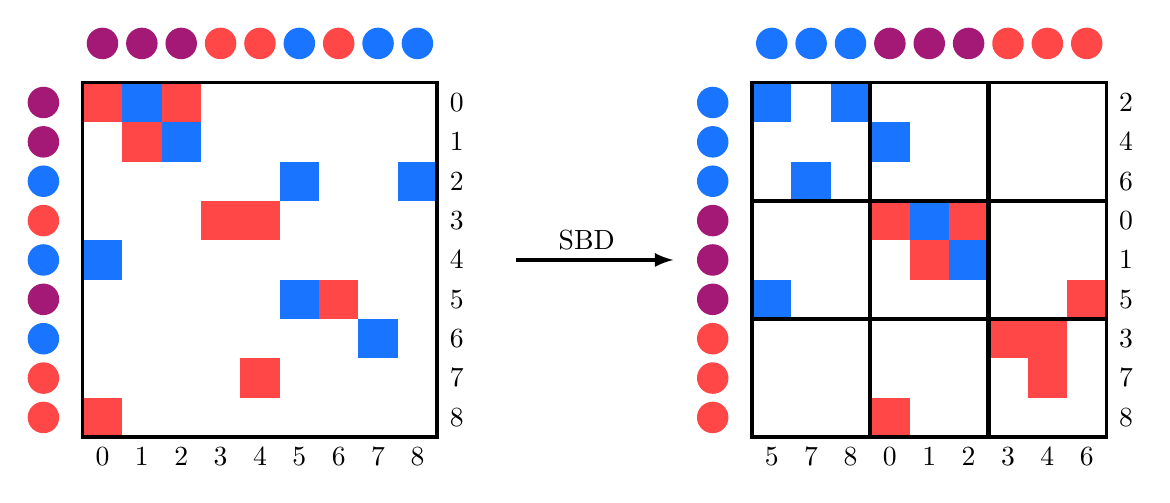
\begin{tikzpicture}[scale=0.5]
		\tikzstyle{myred}=[red!90,opacity=.8]
		\tikzstyle{myblue}=[blue!60!cyan,opacity=.9]
		\tikzstyle{mypurple}=[purple!80!blue,opacity=.9]
		\tikzstyle{myarrow}=[line width=1.3pt,>=latex,->]

		\foreach \x / \y in {1/1,1/3,2/2,4/5,4/4,8/5,6/7,9/1} { \fill[myred] ({\y-1},{-\x+1}) rectangle +(1,-1);}
		\foreach \x / \y in {1/2,2/3,3/6,3/9,6/6,5/1,7/8} { \fill[myblue] ({\y-1},{-\x+1}) rectangle +(1,-1);}
%		\draw[help lines] (0,-9) grid (9,0);
		\foreach \x in {0,1,...,8} {\node at ({9.5},{-\x-.5}) {\x};}
		\foreach \x in {0,1,...,8} {\node at ({\x+.5},-9.5) {\x};}


		\foreach \x in {1,2,3} { \fill[mypurple] ({\x-0.5},1) circle (0.4cm);}
		\foreach \x in {4,5,7} { \fill[myred] ({\x-0.5},1) circle (0.4cm);}
		\foreach \x in {6,8,9} { \fill[myblue] ({\x-0.5},1) circle (0.4cm);}

		\foreach \x in {1,2,6} { \fill[mypurple] (-1,{-\x+0.5}) circle (0.4cm);}
		\foreach \x in {4,8,9} { \fill[myred] (-1,{-\x+0.5}) circle (0.4cm);}
		\foreach \x in {3,5,7} { \fill[myblue] (-1,{-\x+0.5}) circle (0.4cm);}

		\draw[very thick] (0,-9) rectangle (9,0);

		\draw[thick,myarrow] (11,-4.5) -- (15,-4.5);
		\node at (12.8,-4) {SBD};
		\foreach \x / \y in {4/4,4/6,5/5,7/8,7/7,8/8,6/9,9/4} { \fill[myred] ({17+\y-1},{-\x+1}) rectangle +(1,-1);}
		\foreach \x / \y in {1/1,1/3,2/4,3/2,4/5,5/6,6/1} { \fill[myblue] ({17+\y-1},{-\x+1}) rectangle +(1,-1);}

%		\draw[help lines] (17,-9) grid ({17+9},0);
		\foreach \x / \y in {2/0,4/1,6/2,0/3,1/4,5/5,3/6,7/7,8/8} {\node at ({17+9.5},{-\y-.5}) {\x};}
		\foreach \x / \y in {5/0,7/1,8/2,0/3,1/4,2/5,3/6,4/7,6/8} {\node at ({17+\y+.5},-9.5) {\x};}


		\foreach \x in {4,5,6} { \fill[mypurple] ({17+\x-0.5},1) circle (0.4cm);}
		\foreach \x in {7,8,9} { \fill[myred] ({17+\x-0.5},1) circle (0.4cm);}
		\foreach \x in {1,2,3} { \fill[myblue] ({17+\x-0.5},1) circle (0.4cm);}

		\foreach \x in {4,5,6} { \fill[mypurple] ({17-1},{-\x+0.5}) circle (0.4cm);}
		\foreach \x in {7,8,9} { \fill[myred] ({17-1},{-\x+0.5}) circle (0.4cm);}
		\foreach \x in {1,2,3} { \fill[myblue] ({17-1},{-\x+0.5}) circle (0.4cm);}

		\draw[very thick] ({17+0},-9) rectangle ({17+9},0);

		\draw[ultra thick] ({17+3},0) -- ({17+3},-9);
		\draw[ultra thick] ({17+6},0) -- ({17+6},-9);

		\draw[ultra thick] ({17+0},-3) -- ({17+9},-3);
		\draw[ultra thick] ({17+0},-6) -- ({17+9},-6);
	\end{tikzpicture}
	\caption{Example of SBD form of a partitioned matrix. On the left the original matrix is shown whereas on the right we have the permuted SBD form. On the top/left sides of the matrices it is shown whether that row is completely red or blue or it is mixed (purple), whereas on the bottom/right sides the indices of the columns/rows are explicitly given.} \label{fig:sbd}
\end{figure}

If we denote with $P_{\pi}$ and $P_{\sigma}$ the permutation matrices obtained from $\pi$ and $\sigma$, we have that the resulting permuted matrix is the following block tridiagonal matrix:

\[ \tilde{A} := P_{\pi} A P_{\sigma} = 
	\begin{bmatrix}
		\tilde{A}_{00} & \tilde{A}_{01}  & \\
		\tilde{A}_{10} & \tilde{A}_{11} & \tilde{A}_{12} \\
		& \tilde{A}_{21} & \tilde{A}_{22} \\ 
	\end{bmatrix},
\]

where

\begin{itemize}
	\item $\tilde{A}_{00}$ has nonzeros with uncut rows and uncut columns for processor 0;
	\item $\tilde{A}_{22}$ has nonzeros with uncut rows and uncut columns for processor 1;
	\item $\tilde{A}_{01}$ has nonzeros with uncut rows for processor 0, and cut columns;
	\item $\tilde{A}_{21}$ has nonzeros with uncut rows for processor 1, and cut columns;
	\item $\tilde{A}_{10}$ has nonzeros with cut rows and uncut columns for processor 0;
	\item $\tilde{A}_{12}$ has nonzeros with cut rows and uncut columns for processor 1;
	\item $\tilde{A}_{11}$ has nonzeros with cut rows and columns.
\end{itemize}

Note that the size of the blocks (and the quantity of nonzero in them) can vary tremendously: if the sparsity pattern of the matrix allows a ``perfect'' partitioning such that there is no communication, all blocks are empty except of $\tilde{A}_{00}$ and $\tilde{A}_{22}$, whereas if the matrix has a very dense (or complicated) pattern and/or the partitioning is lousy, we might have such blocks almost empty and the central block $\tilde{A}_{11}$ with the majority of nonzeros. An example of this difference is shown in Figure \ref{fig:sbd-2}.

\begin{figure}[h]
	\centering
	\subfigure[\texttt{impcol\_b}]{ 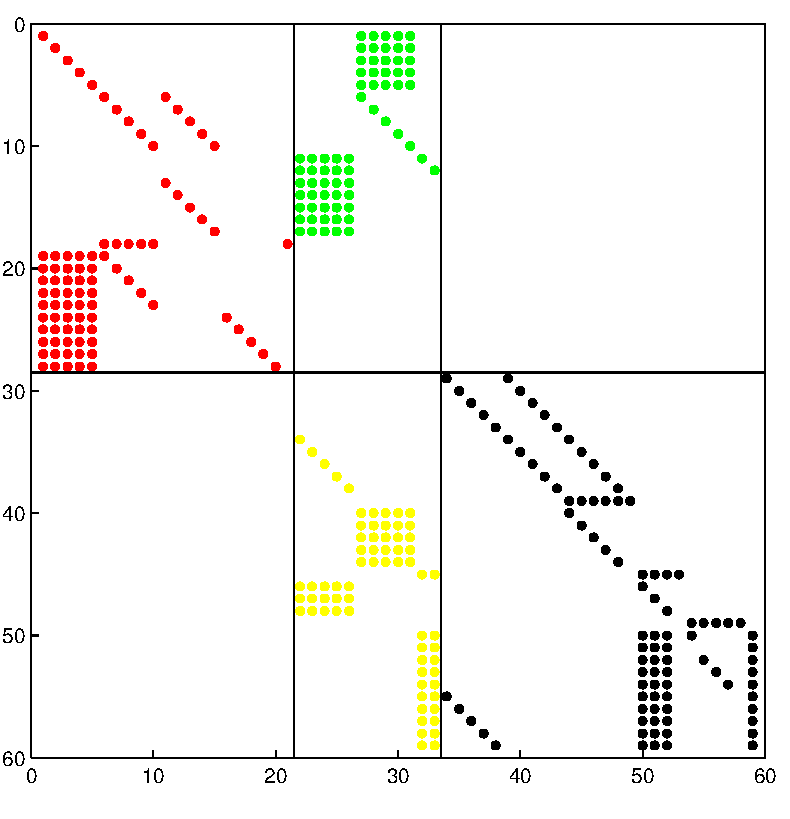
\includegraphics[scale=0.4]{img/impcol_b.pdf} \label{fig:impcol_b}} \hspace{1cm}
	\subfigure[\texttt{cage7}]{ 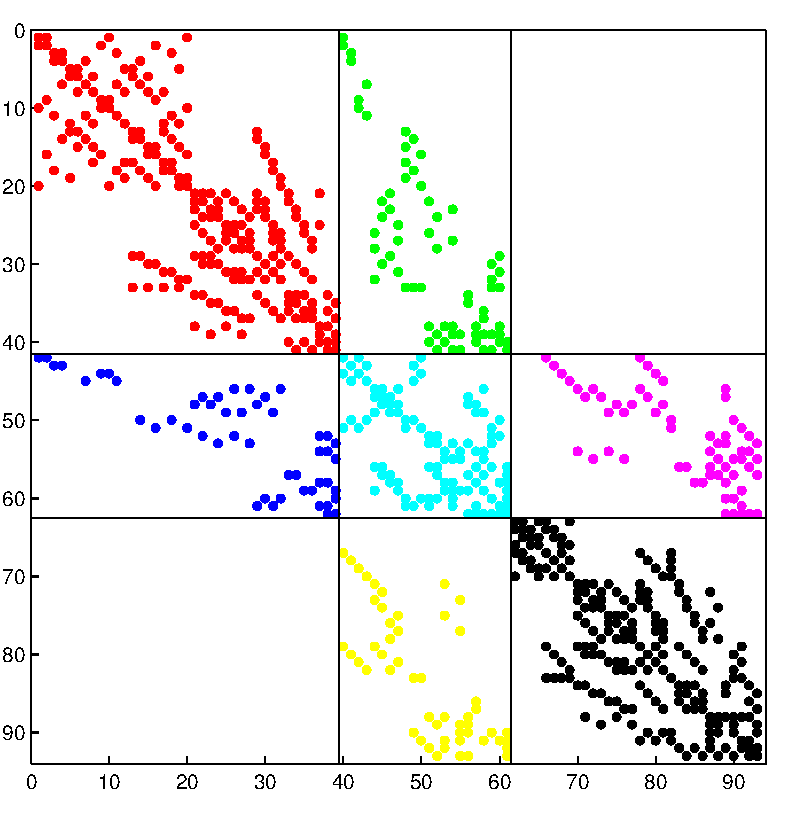
\includegraphics[scale=0.4]{img/cage6.pdf} \label{fig:cage6} }
	\caption{Example of SBD forms of partitioning of the matrices \texttt{impcol\_b} and \texttt{cage6}. Each part of $\tilde{A}$ has been colored differently. In the first matrix there are no cut rows, and therefore $\tilde{A}_{10}=\tilde{A}_{11} =\tilde{A}_{12} = \varnothing$. The images were produced with MATLAB.} \label{fig:sbd-2}
\end{figure}



We can exploit the structure of this matrix $\tilde{A}$ and adopt rule for the assignment of each of its blocks.

\section{Maximizing empty rows of $B$} \label{sec:globalview}

At the beginning of this chapter we mentioned how it is convenient to have full rows assigned to $A_r$ and full columns assigned to $A_c$, in order to avoid communication; a good strategy to produce good $A_r$ and $A_c$ could then be to maximize such full assignments.

The proposed heuristic does substantially this: instead of a generating scheme, it is more of an improvement scheme and, given $A_r$ and $A_c$, it tries to move around nonzeros in order to obtain full rows assigned to $A_r$ and full columns to $A_c$, by considering nonzeros that belong to rows and columns that are both cut. If we change the assignment of those nonzeros, we are sure to not increase the communication volume, while there is still the possibility of decreasing it. 

To have a unique formulation that can obtain full rows assigned to $A_r$ and full columns to $A_c$, it is convenient to reason in terms of the resulting matrix $B$, obtained following the medium-grain model. If we maximize the number of empty rows of $B$, we are effectively emptying rows of $A_r^T$ (which means emptying columns of $A_r$) and of $A_c$. 

\section{Partial assignment of rows and columns} \label{sec:hot_restart}
